\documentclass{article}
\usepackage[utf8]{inputenc}
\usepackage[margin={.95in,.75in}]{geometry}
\usepackage{titlesec}
\usepackage{titling}
\usepackage[default,scale=1]{opensans}
\usepackage{graphicx}
%\graphicspath{ {./} }

\setlength{\parindent}{0em}
\setlength{\parskip}{0.5em}
\renewcommand{\baselinestretch}{1.5}
%\pagenumbering{gobble}

\author{Ryan Bruno}
\date{\today}
\renewcommand{\maketitle}{

\begin{center}
\setlength{\parskip}{0em}
GEOGRAPHY 140:  CULTURAL GEOGRAPHY

Maps and the Media
\end{center}
\textbf{\underline{Name:}}
\theauthor

\textbf{\underline{Bibliographic Citation:}}

\setlength{\parindent}{10ex}
Parletta, Natalie. 2019. World map rates sustainable food systems. \textit{Cosmos}. Nov. 27.
\setlength{\parindent}{0ex}
}

\begin{document}

\maketitle

\textbf{\underline{Analysis}}

\setlength{\parindent}{10ex}
The map found on the next page is a map rating the sustainability of the food system of every country. The scale goes from blue to red, high to low respectively, and grey is given to countries with insufficient data, most notably China. The map was found accompanying an online version of a magazine article. The article gives more context to the map; most importantly adding that the metrics took into account environmental impact, health and food security, social equity, and income distribution. The food system of a country can tell us a lot about the country. When you combined all parts of the global food system it is the world's biggest employer and tracking the sustainability of each countries food system can tell about that countries development. The article also adds that the map is designed for benchmarking and monitoring. In my opinion, it does a good job of this.

The maps colors give the views a quick reference of a countries sustainability but you can analyze it a little deeper. As expected most developed countries are blue such as the US, Australia, and all of the EU. Similarly, developing countries are red. India is a good example of a developing country that this map tells us is behind in food system sustainability. We can analysis deeper, adding that India has a very high population compared to its land size, making sustainability harder. On top of that, we can see a trend in food system suitability and latitude. Regions such as Northern Africa and Central America are harder to grow crops in, which explains their low sustainability score. On the flip side, the developing nations in South America have relatively high sustainability scores because it is easier to grow crops. One country who is marked as insufficient data that I would have liked to analyze is China. There has been some debate recently if they should be considered a developed country yet and having their data would help with that debate.

From the article, you can tell that the target audience of the map was not children neither was it for experts in the sustainability field. It was targeted to anyone who can critically analyze a map and would like an overview of the relative sustainability for each countries food system. It provides a way for the reader to quickly reference and analyze the map. In the future, another article can be published displaying both this map and an updated version of the map. For the reader, it would be very easy to compare the two and tell whether a country improved or not. 

This map sparks an interesting question. Should wealthy nations help nations who have an unsustainable food system? A wealthy nation could continue to improve its food system until it is truly sustainable or help others get to the same level as them. It is hard to enlist help from other nations but the damage done to the environment from one country's food system could affect others.

\setlength{\parindent}{0ex}
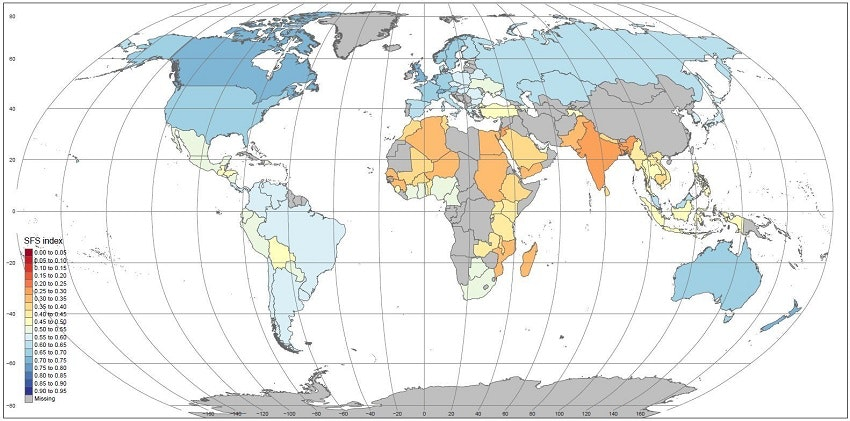
\includegraphics[width=\textwidth]{map}

\end{document}
